\documentclass[]{report}

\usepackage{graphicx}
\usepackage{bookmark}

\usepackage{multirow}
\usepackage[table,xcdraw]{xcolor}

% Title Page
\title{Technical Manual \newline Yavin IV Defence System}
\author{Team Dirac}


\begin{document}
\maketitle

\chapter{Introduction}
\section{Document Identification}
This document describes the design and development of the "Yavin IV Orbital Tracking System".  This document and design brief is prepared by Dirac Defence Limited for assessment in MTRX3700, year 2014. The was approved by lieutenants Reid and Bell, and small scale testing initiated. 

\section{System Overview}
%A brief statement of the purpose of the system or subsystem to which this document applies.

This document outlines a proposed and prototyped design in response to the Rebel Alliance Commander Rye's request for a defence system to combat the imminent threat posed by The Empire, and their Death Star weapons platform. This system is to effectively, efficiently and easily track a space-based planetary annihilator, approximately the size of a small moon.\newline
The system described in this paper is the small scale prototype for stage one of implementation and testing prior to contract approval and large scale deployment. IV Defence System is designed to provide accurate, low cost tracking for Death Stars and other similar objects.

\section{Document Overview}
%A short “road map” of the document, to provide an orientation for the reader. Summarise the purpose and contents of this document.

This technical document provides a detailed description of the design process and requirements of the various modules of the Orbital Tracking System. \newline

Section one provides the main body of the technical document and outlines the development process of the system.\newline
Chapter one introduces the system and document, details the technical jargon used and addresses reference documents used. \newline
Chapter two describes the system requirements, operational scenarios, module design and module requirements. \newline
Chapter three details the user interface design and interactions with different user classes. \newline
Chapter four specifies the hardware design, validation and maintenance. \newline
Chapter five details the software design process, architecture and preconditions for use. \newline
Chapter six describes the performance of the system and future development. \newline
Chapter seven outlines the safety implications of the system. \newline
Chapter eight addresses conclusions and provides final final analysis of the system. \newline

Section two contains the supporting documents, calculations, DOxygen documentation and code listings.

\section{Reference Documents}
The present document is prepared on the basis of the following reference document, and should be read in conjunction with it.\newline 

"MTRX3700 Mechatronics 3, Major Project: Multi Sensor Death Star Tracker".  David Rye, Sydney, 2014.
\subsection{Acronyms and Abbreviations}

\begin{center}
	\begin{tabular}{| l | c |}
		\hline
		Acronym & Meaning \\ \hline \hline
		OTS & Orbital Tracking System, the system under development \\ \hline
		ADC & Analogue-to-Digital Converter \\ \hline
		Stuff & Meaning of Stuff \\
		\hline
	\end{tabular}
\end{center}

\chapter{System Description}
This section is intended to give a general overview of the basis for the Yavin IV Defence System system design, of its division into hardware and software modules, and of its development and implementation.

\section{Introduction}
%Give a technical description of the function of the whole system, in terms of its constituent parts, here termed modules. Generally, a module will have hardware and software parts.

The Yavin IV Orbital Tracking System's primary function is to track the Galactic Empire's Death Star system in real-time. 
It consists of the following two major modules, tracking and user interface.


Tracking
This module takes data from the range and pan-tilt modules
unfinished

-Range
--Ultrasound 
--Infrared
--Temperature

--Pan-Tilt

Menu System
--LCD
--Local User Interface
--Serial

\section{Operational Scenarios}
%Describe how the system is to be used. There may be several different ways that it ca be used perhaps involving different users, or classes of user. Present case diagrams here if you are using them. Each operational scenario is a part through a use case diagram - a way of using the system, with different outcomes or methods of use. You should also consider the various failures that may occur, and the consequences of these failures. 

The system is designed to work in two different modes depending on the class of user, factory mode and end-user mode.\newline
The end user mode is primarily designed to be implemented as the main operational mode, and offers automatic and manual tracking, serial and local user input and output. The factory mode allows technically trained users to calibrate various settings, change sample rates, show statistics and display raw readings, in addition to the full functionality available in end user mode.\newline
Prior to distribution, the system will be calibrated in factory mode and upon distribution, the system will be initialised in user mode. This is to ensure the system is in optimal operating condition and so that the user may not inadvertently modify critical settings. \newline
The factory mode is protected by a physically isolated electrical line and may be initialised by inserting and turning the factory key.

\section{System Requirements}
The operational scenarios considered place certain requirements on the Yavin IV Defence system, and on the modules that comprise it.

The system's primary objective is to locate and track an enemy deathstar, then provide relevant information corresponding to its whereabouts via a serial and local interface. The secondary requirements are the system is to be powered by a 9V PP3 DC battery, implemented on a Microchip PIC18F4520 micro-controller, programmed in "C" language and/or natural assembly language, peripheral electronics shall be constructed on veroboard.  
%Statement of requirements that affect the system as a whole, and are not restricted to only a subset of its modules.

\section{Module Design}
<Describe the breakdown of the design into functional modules. Each module probably contains both software and hardware.
Then include a section like the following 2.5 for each module. Not all of the sub-headings may be relevant for each module.>

The system was broken down into a number of independent modules which contain their own private variables, functions etc. Fig. \ref{fig:Modules} gives an approximate diagrammatic representation of the way the modules fit together.

\begin{figure}
\centering
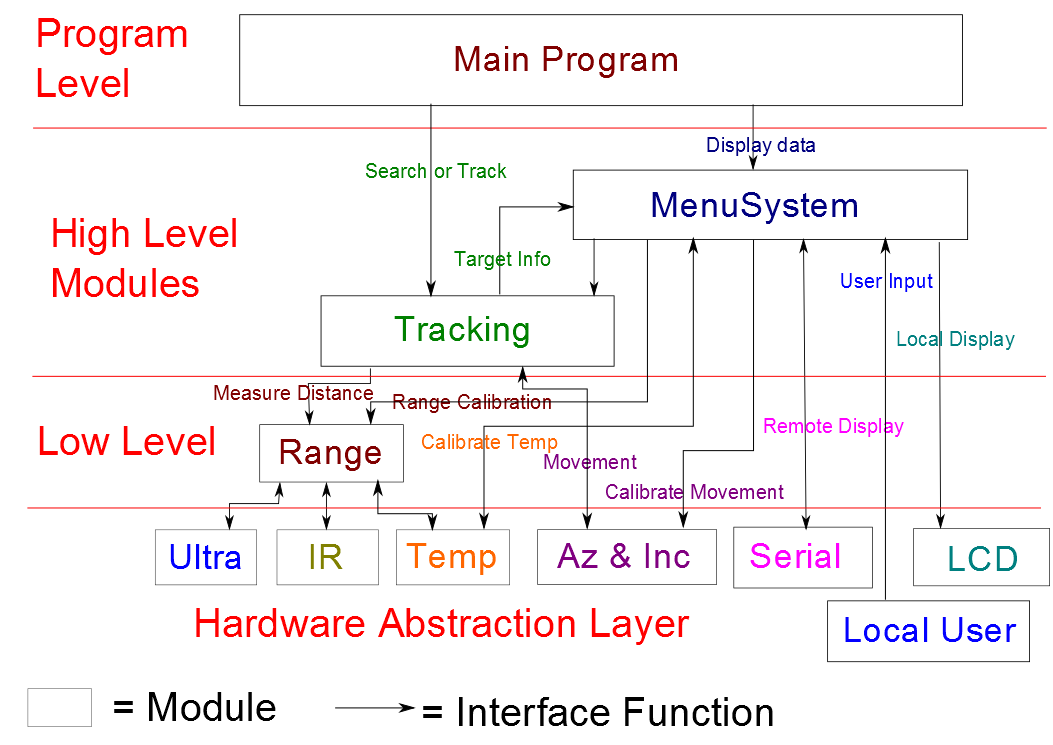
\includegraphics[width=0.7\linewidth]{../Diagrams/Modules}
\caption[Modules]{Conceptual Diagram of the module breakdown and interaction between modules.}
\label{fig:Modules}
\end{figure}



\section{Module Requirements: Serial}

\subsection{Functional Requirements}
\subsubsection{Inputs}
The module must be capable to receiving characters from a user program and transmitting them over serial. The ability to send strings is considered an extension of the basic functionality. \newline
The system must be capable of receiving and storing characters over the serial line, and reporting them back to the user program when requested.

\subsubsection{Processes}
The module must be capable of performing the following processes:
\begin{itemize}
	\item Receiving data over serial line
	\item Sending data over serial line
	\item Storing data to be transmitted
	\item Storing data received
	\item Interface with the user program
\end{itemize}


\subsubsection{Outputs}
The module must be capable of returning the following outputs:
\begin{itemize}
	\item exact characters received over the serial line in the correct order.
	\item Whether the system has received anything
	\item Data Characters over the serial line
\end{itemize}

\subsubsection{Timing}
The serial module must be capable of:
\begin{itemize}
	\item Storing characters as soon as they are received over serial
	\item Retaining received characters until they are handled
	\item Retaining transmission characters until they can be transmitted
\end{itemize}

\subsection{Non-Functional Requirements}
\subsubsection{Performance}
The serial module should have the following performance characteristics:
\begin{itemize}
	\item Very fast ISR's - to affect background code, and other waiting interrupts as little as possible
	\item Very low ISR latency - So no characters are missed, and the the module transmits almost as soon as possible.
\end{itemize}

\subsubsection{Interfaces}
The following interface requirements are desirable:
\begin{itemize}
	\item Complete isolation/modularisation (e.g. no global interrupts) - the buffers are not accessible to the rest of the program
	\item Very simple, intuitive interface functions taking 1 or no arguments that are appropriately named.
	\item As simple operation as possible - E.g. configureSerial() then transmit().
\end{itemize}

\subsubsection{Design Constraints}
The design of the serial module was constrained by the following:
\begin{itemize}
	\item Only High and Low ISR's on the PIC - Needed a public ISR function that is called when a serial interrupt is fired - Reduced modularity and interrupt response
	\item Very little memory on the PIC - buffers were restricted to 30 characters
\end{itemize}

\section{Conceptual Design: Serial}
\subsection{Description}
The serial module takes care of all communication (transmit and receive) over the serial UART (rs-232) port.

\subsection{Overall Design}
The serial module was designed to be as simple and intuitive to use as possible. For this reason the final design ended up being very similar to the serial on an arduino. \newline
There are two inbuilt circular buffers: a transmit buffer and a receive buffer. Any inputs to the serial module for transmission are simply placed into the transmission buffer to be transmitted at the next available opportunity. Any data received over serial is automatically pushed onto the receive buffer to be used by the program. \newline
The buffers are completely hidden from the rest of the program, and the user simply interacts with the buffers in an intuitive manner to send and receive data

\subsection{Detailed Description}
The serial module is INTERRUPT DRIVEN. This means that any background code can be running while the module is transmitting and/or receiving data over the serial line, and no serial data should ever be missed, overlooked or cut out. \newline
The module contains two circular buffers: a transmit buffer and a receive buffer. These buffers are NOT accessible by the rest of the program. Rather, the module provides a public function transmit() which takes a string, and places it into the transmit buffer. Anything in this buffer is then transmitted character by character when the transmit ready interrupt fires. \newline
Whenever a character is received over serial it is stored in the received buffer by an interrupt. Again this buffer is NOT accessible to the rest of the program. Rather it provides a number of functions to interact with it. The most commonly used of which is the readString() function, which returns everything in the buffer up to a carriage return (e.g. a line of input entered by the user). \newline
This serial module also allows users the opportunity to remove or change data they have already transmitted. If a backspace is received, then instead of storing it in the receive buffer it will remove the last received character from the buffer if that character is not a Carriage Return, Newline, or Escape operator. This enables a much more more user friendly system as otherwise there would be no way to fix any syntax error without pressing enter, getting an error and starting again. Furthermore, without this feature, if a user did backspace and change an input it would result in completely unexpected behaviour. \newline
Fig. \ref{fig:SerialModule} shows a conceptual diagram of the function of the serial module.

\begin{figure}
	\centering
	\includegraphics[width=0.7\linewidth]{"../Diagrams/Serial Module"}
	\caption[Serial Module]{Shows Conceptual Diagram of Serial Module -> Received input stored by interrupts into circular buffer to await pop commands. Transmit data pushed onto buffer which is transmitted via interrupts}
	\label{fig:SerialModule}
\end{figure}

\subsection{Rational for Design}
The rational for the serial module is fairly self explanatory: any decent serial module requires buffers to help prevent data loss, with the ideal implementation being circular buffers. The buffers are kept isolated for modularity and good programming practise, while it also serves to greatly simplify the usage and novice users are not confused by access to buffers and other data structures. The rest of the interface was then chosen to be as simple and intuitive as possible.

\subsection{Implemented Functionality}
\subsubsection{Implemented Basic Functionality}
The serial module implements the following basic functionality:
\begin{itemize}
	\item Functioning receive and transmit serial interrupts
	\item Configure function to set up the module
	\item Separate circular buffers to store data received and data to be transmitted
	\item Public Function to add data to the transmission buffer
	\item Public Function to read from received buffer, and check if anything has been received
\end{itemize}


\subsubsection{Implemented Additional Functionality}
In addition to the required functionality above, the serial module also offers the following functionality:
\begin{itemize}
	\item Push Null terminated strings to the transmit buffer
	\item Check if carriage return, or esc has been received
	\item Pop an entire string from the receive buffer up to a carriage return
	\item Clear the buffers
	\item Receiving backspace characters removes the last characters from the buffer (if not CR or ESC)
	\item Read a string form program memory and transmit
	\item Peek - Read character without removing from buffer
	\item Indicate if transmit buffer is empty (all messages sent)
\end{itemize}

\subsection{Assumptions Made}
The module assumes that the buffers will never be overfilled, i.e. is able to transmit data faster than being written into buffer, or that input is being handled in a timely fashion. Failing this, it is assumed that the oldest data (which is overwritten) is the least meaningful, and that loosing some data will not create catastrophic error in the system. It is recommended to include a wait if sending large blocks of text over serial.

\subsection{Constraints on Serial Performance}
The main constraints on the serial module performance are:
\begin{itemize}
	\item Baud Rate
	\item Interrupt Latency
\end{itemize}
The baud rate sets a maximum rate data can be transferred, which along with the buffer length restricts the rate at which data can be written to the transmit buffer without an overflow occurring.
The interrupt latency is the time delay between the interrupt firing and the actual event. This is generally very small (we found ~300$\mu$s), but a high latency could miss characters being received.

\subsection{Interface}
Refer to the Technical User Manual For detailed explanations of the interface functions and how to use them.

\subsubsection{List of inputs}
The following are inputs that can be sent to the serial module for transmission:
\begin{itemize}
	\item Strings (RAM char array) through transmit()
	\item Strings (ROM char array) through sendROM()
	\item Characters through transmitChar()
\end{itemize}

In addition, the serial module has serial input from whatever terminal it is communicating to. This is via TTL level logic rs-232 at 9600 baud. The terminal communicates at rs-232 level logic, which is then converted by an adapter on the minimal board.

\subsubsection{List of Outputs}
The following are outputs that can be requested from the serial module following reception:
\begin{itemize}
	\item Characters from receivePop(), receivePeek()
	\item Strings from readString()
\end{itemize}

The serial module also outputs TTL level logic at 9600 baud rs-232 encoding which is then converted to rs-232 level logic to the terminal.



\section{Module Requirements: Pan Tilt}

\subsection{Functional Requirements}
\subsubsection{Inputs}
The Pan Tilt module must be capable of taking the following inputs:
\begin{itemize}
	\item The desired direction
\end{itemize}

\subsubsection{Processes}
The Pan Tilt module must be capable of performing the following processes:
\begin{itemize}
	\item Storing the current direction\\PDM
	\item Converting a given direction into a PDM
	\item Continuously generating the control PDM to send to the servo motors
\end{itemize}

\subsubsection{Outputs}
The program must be capable of the following outputs:
\begin{itemize}
	\item PDM control signal to the servo's
	\item Current direction back to the user program
\end{itemize}

\subsubsection{Timing}
The Pan Tilt module must conform to the following timing specifications:
\begin{itemize}
	\item Module must be interrupt driven
	\item Must have very low interrupt latency
	\item PDM's must be offset so that the interrupts for elevation and azimuth don't interfere and block each other
	\item Delay after movement function to allow the servo's to move to that position
\end{itemize}

\subsubsection{Failure Modes}
The Pan Tilt module includes the following assurances against failure:
\begin{itemize}
	\item New delay information is only set at the end of a cycle to guarantee the PDM frequency
	\item Validation function to ensure that the high time to within the specified range in the datasheet  
\end{itemize}

\subsection{Non-Functional Requirements}
\subsubsection{Performance}
The module should have the following performance characteristics to perform well:
\begin{itemize}
	\item Very low interrupt latency
	\item Adjustment for interrupt latency
\end{itemize}

\subsubsection{Interfaces}
The following interface characteristics are desirable:
\begin{itemize}
	\item Complete Isolation/modularity so that the rest of the program does not have access to any of the functionality of the module, but merely sets the direction of the Pan-Tilt module
	\item Very simple, intuitive interface functions taking 1 or no arguments that are appropriately named.
	\item Very simple module operation, such as configuration and move to desired location
\end{itemize}

\subsubsection{Design Constraints}
The design of the Pan Tilt module was primarily constrained by the use of the input capture CCP1 for the ultrasonic sensor to capture the return signal. This meant that the remaining CCP module had to be used to generate both PDM's, which could only be done in software. Had an additional CCP module been available, we could have used the hardware PWM mode, which would give much better precision and guarantee in the generation of the PDM's as there would be no influence from software interrupt latency. Also this would make the design much simpler.

\section{Conceptual Design: Pan Tilt}
\subsection{Description}
The Pan Tilt module is responsible for interfacing and driving the pan tilt mechanism. This primarily consists of generating the PDM signals required to send dictate the position of the servo's.

\subsection{Overall Design}
The overall design of the system is to convert any inputted direction into a set of delays required to generate the PDM's. These PDM's are then realised by timing interrupts running off the calculated delays.

\subsection{Detailed Design}
This module uses a single output compare module to create the delays necessary to generate the PDM's of the desired duty cycle. Due to the interrupt latency of approximately 300$\mu$s, the PDM's are staggered so that the interrupt calls will never be closer than approximately 0.04 seconds. The full available duty cycle (1000$\mu$s) is divided over the given angular range. There is also an angular offset for calibration reasons. The Delay object is then created to define the necessary delays to create the desired PDM.
NOTE: This module is interrupt driven, so the Interrupt.c file must be included in the project for it to work. \newline
A data Flow diagram of the Pan Tilt Module is shown in Fig. \ref{PanTiltPins}. \newline
The conversion from inputted angle to outputted PDM delay is simply to divide the full high time (1000$\mu$S to 2000$\mu$S) over a stored angular arc. The angular arc along with a reference offset completely define the calibration of he pan tilt mechanism. \newline
The dataflow through the pan tilt module is depicted in Fig. \ref{fig:PanTiltDataFlowDiagram}.

\begin{figure}
\centering
\includegraphics[width=0.7\linewidth]{"../Diagrams/Pan Tilt Data Flow Diagram"}
\caption[Pan Tilt Dataflow Diagram]{Dataflow diagram showing the transition from inputted direction to servo direction}
\label{fig:PanTiltDataFlowDiagram}
\end{figure}

\subsection{Implemented Functionality}
\subsubsection{Implemented Basic Functionality}
The Pan Tilt module includes the following basic functionality:
\begin{itemize}
	\item Configure function to set up the module
	\item Move function to move to any valid position
	\item Get Direction function to return the current direction
\end{itemize}

\subsubsection{Implemented Additional Functionality}
The following additional functionality has been implemented for the Pan Tilt Module
\begin{itemize}
	\item Incremental move function
	\item Increment fine function for greater precision
	\item Updated function to indicate whether a new delay setting has actually been written into the system yet
\end{itemize}

\subsection{Assumptions Made}
The largest assumption made is that the clock frequencies in the code match those of the actual clock. Common.h defines the clock frequencies of the PICDEM and Minimal Boards which can be switched between. But there is no way for the system to verify the frequency of the clock, and if the clock is not the same then the PDM frequency will not be 50Hz, which can damage the servo's if faster. \newline
The module does not assume that the interrupts fire instantly after the timing event, but that there is an approximately constant latency time, which is found experimentally, included as a \# define, and tuned.

\subsection{Constraints on Pan Tilt Performance}
The Pan Tilt module is restricted to the servo range of motion. Also the actual position is entirely dependant on the calibration as they merely take a PDM input.

\subsection{Interface}
Refer to the Technical User Manual For detailed explanations of the interface functions and how to use them.

\subsubsection{List of Inputs}
The Pan Tilt Module takes the following inputs:
\begin{itemize}
	\item Absolute Direction to which to move (as Direction struct)
	\item Incremental Direction in which to move (as Direction struct)
	\item Calibration Directions (as direction structs)
	\item Configurable system settings as chars
\end{itemize}

\subsubsection{List of Outputs}
The Pan Tilt Module returns the following outputs:
\begin{itemize}
	\item The current direction (as Direction struct)
	\item Position commands to servo's (as PDM's)
	\item Current configurable system settings values (as chars)
\end{itemize}

\section{Range}
\subsection{Description}
The range module uses the IR, Ultrasonic and temperature sensors to take range measurements.

\subsection{Hardware}
The range module makes use of the following hardware:
\begin{itemize}
	\item 600 series Polaroid Ultrasonic range sensor
	\item TL851 Sonar Ranging Control
	\item Infra Red range sensor
\end{itemize}

\subsubsection{Pin Assignments}


\subsection{Functional Requirements}
\subsubsection{Inputs}
The range module takes no real inputs

\subsubsection{Processes}
The range module requires the following processes to function properly
\begin{itemize}
	\item Sample the Ultrasonic and IR sensors
	\item Convert the sensor output to a range
	\item Fuse the ranges from different sensors 
\end{itemize}

\subsubsection{Outputs}
The output of the range module is the range to the target (in mm) as an unsigned int. The module also returns the state of the detected target as an enumeration.

\subsubsection{Timing}
The range module uses an input capture module to record the precise time the ultrasonic echo signal returns, which is then used for the range calculation. An interrupt is then used to indicate that the echo has returned, but precise timing for this is not required, as the echo return is stored in hardware when the echo is detected. 

\subsubsection{Failure Modes}
The system waits for the echo signal to return, but there is a possibility that the echo will never return. For this reason the system has a timeout feature so that if the signal does not return within a specified timeout then the range module returns nothing found. This means that the range module does not get stuck in the range module waiting for the echo signal to return.

\subsubsection{Implemented Basic Functionality}
The range module implements the follow functionality:
\begin{itemize}
	\item Configure the range module
	\item Return the range to the target
\end{itemize}

\subsection{Non-Functional Requirements}
\subsubsection{Performance}

\subsubsection{Interfaces}
Refer to the Technical Users Guide for a detailed explanation of the module interface

\subsubsection{Implemented Additional Features}
The range module also implements the following additional functionality
\begin{itemize}
	\item Fuse the ranges taking the distance into account - US better for long ranges, IR better for short
	\item Categorise the target state based on which sensors return a reading
	\item Range calibrating functions
\end{itemize}

\subsection{Conceptual Design}
The Ultrasonic sensor is interrupt driven, which means that we can be performing other actions while waiting for the echo return. Thus the system uses this time to sample the IR and temperature. The module also allows any number of ultrasonic samples per range estimate, and the IR sensor is sampled continuously while the ultrasonic sensor is being sampled. The module also fuses the ranges returned by the respective sensors based on the range, so that IR is used more at short ranges, and not at all at long ranges. The module also sets a target state that can take a number of states depending on which sensors detect a target. This means the module can differentiate between when the sensors are within the Ultrasonic cone, but not in the IR, or when it is within the Ultrasonic cone, but out of IR range. This is then used for the searching and tracking. 

\subsubsection{Assumptions Made}

\subsubsection{Interface}


\section{Interrupts}
\subsection{Description}
The PIC18F4520 has 2 ISR's, so an interrupt framework whereby each module defines an ISR function, and a macro which determines whether to call its ISR function. The ISR's are then included in their own file, and included here as a semi-module

\subsection{Functional Requirements}
\subsubsection{Inputs}
For the interrupt framework to function each module must define a macro which checks the interrupt flags for all the interrupts associated with the module.

\subsubsection{Processes}
The interrupt framework must be capable of performing the following processes:
\begin{itemize}
	\item Check each module interrupt macro
	\item Ability to call the associated function depending on macro results
\end{itemize}

\subsubsection{Outputs}
The interrupt framework has no real outputs, but directs program execution to the appropriate module ISR

\subsubsection{Timing}
There are no hard timing requirements for the interrupt framework itself, but the high priority interrupts in particular need to be called as soon after the event as possible.

\subsubsection{Implemented Basic Functionality}
The interrupt framework includes the following basic functionality:
\begin{itemize}
	\item Ability to distribute interrupt execution to any module
	\item Priorities (high and low)
\end{itemize}

\subsection{Non-Functional Requirements}
\subsubsection{Performance}
The following characteristics are desirable for performance reasons:
\begin{itemize}
	\item All interrupts should be as fast and efficient as possible so as to interfere with background code, and other interrupts as little as possible. 
	\item Any extended functionality should be placed into functions not called by the interrupts
	\item Use of priorities to ensure precision for some modules such as the pan tilt which rely on it
\end{itemize}


\subsubsection{Implemented Additional Features}
There are no additional features implemented for the interrupt framework

\subsection{Conceptual Design}
For convenience interrupt macros have been defined in Common.h for each possible interrupt call. Querying one of these macros will return true if that interrupt fired an interrupt. These macros look like: TX\_INT, CCP1\_INT.\newline
Each module defines a macro (in its header file) which indicates which interrupts that module is using, by or-ing together the previously mentioned macros. When an interrupt fires it checks these macros for each module, and if true calls a 'module scope ISR'. These macros look like: SERIAL\_INT, RANGE\_INT etc. \newline
These module scope ISR's are just functions defined within each interrupt driven module, which are called whenever an interrupt associated with that macro is called. Thus these functions act as ISR's for the module without conflicting with anything else in the program.

\subsubsection{Assumptions Made}


\subsubsection{Interface}
There is no public interface for the interrupt framework and nothing can call any of its functions. However other modules must define a macro and a service routine which are used in the interrupt module

\section{Module Requirements: Circular Buffers}
\subsection{Functional Requirements}
\subsubsection{Inputs}
In order to function correctly the circular buffers sub-module must be capable of accepting the following inputs:
\begin{itemize}
	\item characters to push onto a buffer
	\item a buffer to operate on
\end{itemize}

\subsubsection{Processes}
In order to function correctly the circular buffers sub-module must be capable of performing the following processes:
\begin{itemize}
	\item Initialise buffer
	\item Increment and modulus pointers
	\item Push characters
	\item Pop characters
	\item Peek characters
	\item Full and empty checking functionality
\end{itemize}

\subsubsection{Outputs}
To function correctly the circular buffers sub-module must be capable of returning the following outputs:
\begin{itemize}
	\item Characters stored in the buffer
	\item The current filled state of the buffer (full or empty)
\end{itemize}

\subsubsection{Failure Modes}
The circular buffer functionality has some inbuilt safe-guards against accidental misuse such as:
\begin{itemize}
	\item Cannot pop an empty buffer
	\item Pushing full buffer overwrites oldest data
\end{itemize}
Unfortunately the C language does not facilitate private object elements, so the user program could manually alter any elements in the buffer, which could likely result in errors. This could be remedied by making circular buffers a full module, with an actual source file, although this would reduce efficiency.

\section{Conceptual Design: Circular Buffers}
\subsection{Description}
The circular buffers sub-module is a header containing everything required to utilise the circular buffer functionality.

\subsection{Overall Design}
Circular buffers are a mechanism used in several different modules, and for this reason the circular buffer definitions and functionality are included in a sub-module like fashion. This consists only of an include-able header which contains all the struct definitions and macro defines needed to fully utilise the buffers.

\subsection{Detailed Design}
The circular buffers header contains the circularBuffer struct definition, which is essentially an array with head and tail pointers which tell the system where to insert and read from the buffer. The header also defines the BUFFERLENGTH (which can be re-defined), and macros such as incMod to increment and modulus with the BUFFERLENGTH. It then contains all the standard circular buffer functionality such as push, pop, peek, empty functionality in the form of efficient macros, specifically designed to induce as little latency in the serial interrupts as possible. \newline
This implementation of circular buffers overcomes the problem of differentiating between full and empty states by not incrementing the tail pointer if it would coincide with the head pointer, essentially reducing the buffer size by one. \newline
Such a design facilitates speed, while still allowing the entire functionality to be alterable and update-able from a single place.

\subsection{Implemented Functionality}
The circular buffer sub-module implements the following functionality:
\begin{itemize}
	\item incMod
	\item empty
	\item full
	\item peek
	\item push
	\item pop
	\item init - Initialises (clears) the circular buffer
\end{itemize}

\subsection{Interface}
The circular buffers sub-module has no real interface with the entire functionality being defined in the header to be included.

\section{Module Requirements: Temp}
\subsection{Functional Requirements}
\subsubsection{Inputs}
The temp module must be capable of taking the following inputs:
\begin{itemize}
	\item Reference temperature to which to calibrate
\end{itemize}

\subsubsection{Processes}
The temp module must be capable of the following processes:
\begin{itemize}
	\item Configuring the system to sample the temperature
	\item Sampling the temperature sensor
	\item converting the sensor output to celcius
	\item Calibrating the temperature sensor
\end{itemize}

\subsubsection{Outputs}
The temp module must be capable of returning the following outputs:
\begin{itemize}
	\item The temperature in Degrees
	\item The raw temperature in Degrees
\end{itemize}

\subsection{Non-Functional Requirements}
\subsubsection{Performance}
For performance the temperature module stores the last temperature sampled, so that any call to the temperature module can simply return this value, meaning the temperature need only be sampled once a minute or so as the temperature does not vary quickly.

\subsubsection{Interfaces}
Please refer to the attached Module Descriptions document

\section{Conceptual Design: Temp}
\subsection{Description}
The temperature module is responsible for sampling, storing and calibrating the temperature sensor, primarily for the ultrasonic range calculation and user output.

\subsection{Overall/Detailed Design}
The system revolves around the temperature sampling. There is a static offset which is calculated from the calibration function and gets added to any sensor reading. The static variable in the temperature module (storing the last temperature sampled) gets updated every time the temperature is read. Calling the getTemp() function simply returns this value without sampling the temperature.

\subsection{Implemented Functionality}
The temperature module implements the following functionality:
\begin{itemize}
	\item Temperature reading
	\item Calibrating temperature
	\item Raw temperature
	\item configure temp module
\end{itemize}

\subsection{Assumptions Made}
The primary assumption made in the temp module is that the system temperature will not change very quickly, which means that the temperature does not need to be sampled each time the temperature value is used. Instead it simply uses a previously sampled value, and ressamples the temperature at semi regular intervals.

\subsection{Constraints on Temperature Sensor Performance}
The main constraint on the performance of the temperature module is the accuracy of the temperature sensor itself, which is only accurate to within half a degree Celcius. 

\subsection{Hardware}
The temperature module makes use of the following hardware:
\begin{itemize}
	\item Temperature sensor
\end{itemize}
Originally amplifiers were planned to set the analogue to digital converter to the same voltage range as the output of the temperature sensor. But this was deemed unnecessary because the resolution of the ADC was already greater than that of the temperature sensor.

\subsubsection{Pin Assignments}
The following pins are used to connect to the temperature module hardware:
\begin{itemize}
	\item Output of Temp sensor to AN1 Pin
	\item Temp $V_{CC}$ to general purpose 5v bus
	\item Temp GND to common ground
\end{itemize}

\subsection{Interface}
Please refer to the attached Module Descriptions document

\section{Module Requirements: Tracking}
\subsection{Functional Requirements}
\subsubsection{Inputs}
There are no real external inputs to the tracking module, as the functions are iterative they perform a single iteration and return. Thus they are simply called continuously whenever the system is detecting a target. The following inputs are requested by the tracking module from other modules such as range:
\begin{itemize}
	\item Current system state
	\item Target Range
	\item Target State
	\item Pan Tilt Direction
\end{itemize}

\subsubsection{Processes}
The tracking module is required to perform the following processes:
\begin{itemize}
	\item Move the Pan Tilt module in a search pattern
	\item Use sensor data to detect targets
	\item Use algorithms and sensors to track moving targets
\end{itemize}

\subsubsection{Outputs}
The tracking module is required to return the following outputs:
\begin{itemize}
	\item The target details (range, azimuth, elevation)
	\item whether it still has a target
	\item the next system state
\end{itemize}

\subsection{Non-Functional Requirements}
\subsubsection{Performance}
In order to perform well (defined as accurate and reliable track) the system should have the following characteristics:
\begin{itemize}
	\item Quite fast tracing step
	\item Fine adjustments when target is fixed
	\item Coarse adjustments when target is unknown
	\item Efficient tracking algorithm
\end{itemize}

\subsubsection{Interfaces}
The system should have the following interface characteristics:
\begin{itemize}
	\item 
\end{itemize}

\section{Conceptual Design: Tracking}
\subsection{Description}
The tracking module contains the high level tracking and search algorithms used by the system. It then uses the Pan Tilt and Range modules to enact these modules.

\subsubsection{Overall Design}
The searching algorithm uses a simple raster scan variant which scans the azimuthal range, then increments (or decrements) the elevation and scans back the other way. When the system detects any object with either the ultrasonic or the infra red then it enters the tracking mode. \newline
The tracking mode uses a simple weighted average technique, where the system increments the pan tilt direction up, down, left and right of the know target, and averages the directions based on the returns it samples at each of those points. The result is the new target position.

\subsubsection{Detailed Design}
The Tracking module contains two primary functions: search and track. Each of these functions is 'incremental' in nature. This means a single call will perform a single 'step', and these functions are called continuously to perform a constant action. \newline
The search algorithm is based on a simple raster like scan. The system simply increments sweeps the azimuth, incrementing the elevation each time it hits the max or min azimuth. If it gets to the limits of the elevation then it reverses the direction of its increment variable, making the system scan the other way. \newline
As mentioned previously the tracking algorithm is a simple weighted average. The algorithm is highly configurable with surprising ease, but currently it is configured so as to take sampled above, below, to the left and to the right of the know target location. If the system gets an ultrasonic return (i.e. in the large ultrasonic cone) then it assigns a weighting of 1, adding that direction to the sum. If it returns an IR reading it multiplies the direction by 8, and adds it, no return has no weighting. Then it divides by the sum of the weights to get the new target location. \newline
This means that if it is far from the target, then only 1 direction will get returns and the system will necessarily move toward the target. If it is almost on the target, then the preferential return of ultrasonic and/or IR samples to one side will serve to tune the know position.

\subsubsection{Assumptions Made}
There are a number of assumptions made in this module these are as follows:
\begin{itemize}
	\item The searching algorithm does not 'miss' any targets (i.e. scans faster than they can move)
	\item The target is approximately stationary compared to the speed of the tracking algorithm (so that all 5 samples can be considered for the target at a fixed location)
	\item That the sensors do not exhibit any false positives or false negatives
\end{itemize}
Some of these assumptions may seem a little ambitious, however, in a real world scenario they seem to be sufficient to create a working system, albeit not an ideal one.

\subsubsection{Constraints on the Tracking Performance}
Below are some of the more major constraints on the performance of the tracking algorithm:
\begin{itemize}
	\item The maximum sampling rate of the ulrasonic - limited the overall tracking speed
	\item The resolution of the servo's - made it difficult to accurately track distant targets
\end{itemize}

\subsubsection{Hardware}
The tracking system itself made use of no dedicated hardware, it was simply a high level software module, however it did make use of many other modules utilising a range of hardware, such as the range and pan tilt modules.

\subsubsection{Interface}
Refer to the attached Module Descriptions document

\section{Module Requirements: Local User Interface}
\subsection{Functional Requirements}
For a functioning local user interface, the following requirements must be met.
\subsubsection{Inputs}
\begin{itemize}
	\item The user must be able to select options suitable to the system in an intuitive manner. This can be done using a potentiometer, encoder, or left/right buttons. This system uses a potentiometer which the user can rotate to choose an option.
	\item The user must be able to confirm/select their input using a button on the device.
	\item The user must be able to cancel and return from their selection using a button on the device.
	\item The buttons must only trigger a signal once when pressed, and should not incorrectly return a signal. This can be done using a de-bouncing circuit and a pull-down resistor.
\end{itemize}
\subsubsection{Processes}
The Local User Interface module must map the physical actions of the user to software outputs which the menu system can analyse and use. The necessary processes are:

\begin{itemize}
	\item Adding button presses to a circular buffer to be retrieved and handled by the menu system so that order is conserved.
	\item Indicating when the buffer is empty, or contains an escape character. 
	\item Process the potentiometer value from the microcontroller's ADC, and scale the value into discrete steps for a given number of steps.
\end{itemize} 
\subsubsection{Outputs}
\begin{itemize}
	\item The module must be able to indicate when a confirm or escape button is pressed.
	\item The module must be able to indicate which button was pressed, and the order buttons are pressed.
	\item The module must be able to output the converted value from the potentiometer. 
	\item The hardware for the interface must also contain the physical LCD module and the circuitry needed to support it.
\end{itemize}
\subsubsection{Timing and Performance}
The local interface must act immediately when a button is pressed by using an interrupt subroutine, so that user may press buttons as fast as they would like. Readings from the potentiometer must be performed at a fast enough pace so that the user does not notice an unresponsive system. This is usually on the order of approximately 10 samples per second.

\subsection{Non-Functional Requirements}
\subsubsection{Interface}
Aside from functional requirements, there are other requirements for the system to operate the best it can. In terms of hardware, the local user interface must be ergonomic and robust for the user to easily be able to handle the device. The system should also be adequately labelled so that any user can use the system without prior training. 

The software interface must be intuitive, and be based upon the circular buffer module used above. 
\subsubsection{Design Restraints}
The local user interface must be constructed from available and moderately priced components. This is so that different prototypes of the user interface can be constructed cheaply, and in the future if a client is in need of repairs, the time and monetary cost of repairing the device is not expensive. 

As per the other modules, the software for the local interface must be programmed in C and run on the PIC18F4520 microcontroller. Due to the size of this module, it is ideal that the module is lightweight and can be built upon the circular buffer module.

\section{Conceptual Design: Local User Interface}
\subsection{Hardware}
\subsection{Software}


\section{Module Requirements: Menu Subsystem}
\subsection{Functional Requirements}
\subsubsection{Inputs}
The menu subsystem must be capable of taking the following inputs in order to fulfil its purpose:
\begin{itemize}
	\item User inputs from the Serial and Local Interface modules
	\item A pointer to a tracking state to be initialised to, so that the menu can modify or read whether the system is tracking, searching, or waiting for user input.
	\item Inputs from the Range and PanTilt modules for the current value of the system settings that a user can modify. 
	\item Digital logic level from a physical key switch attached to a pull-down resistor circuit to signal Factory mode is to be used. 
\end{itemize}

\subsubsection{Processes}
The menu subsystem must be capable of performing the following processes in order to fulfil its purpose:
\begin{itemize}
	\item The menu system must be able to switch between a local, remote serial and factory serial user mode. 
	\item Parse and convert user data from the Serial and Local User Interface modules into integer values which the menu system and other modules can effectively use. 
	\item Switch to another menu when commanded to by the user.
	\item Convert system values to ASCII messages to display.
	\item Convert messages in the system's ROM memory bank to RAM so that the Serial module can display them. 
\end{itemize}

\subsubsection{Outputs}
The menu subsystem must be capable of returning the following outputs in order to fulfil its purpose:
\begin{itemize}
	\item Messages and structure for the LCD module to display to show the local user interface.
	\item Messages for the Serial module to display to form the serial menus.
	\item Error messages when the user inputs incorrect values.
	\item User input values to the corresponding modules to change system settings. 
\end{itemize}

\subsection{Non-Functional Requirements}
\subsubsection{Performance}
The menu subsystem should have the following characteristics in order to operate efficiently:
\begin{itemize}
	\item The system should be able to quickly respond to user input and quickly display messages, so that the user does not view the system as unresponsive and broken. A response time of 100 milliseconds or less is desired. 
	\item The serial interface for the user must be easy to understand and use commonly used keys or commands. 
	\item The user should be able to intuitively know where options are, and how to navigate between different menus.
	\item The menus should be aesthetically pleasing and consistent between menus. 
\end{itemize}

\subsubsection{Interfaces}
The menu subsystem should have the following interface characteristics in order to operate efficiently:
\begin{itemize}
	\item The menu system must be able to access the functions from the Range and PanTilt modules which can access and change system variables, such as the maximum system range. 
	\item Tracking data from the Tracking module should be easily available to the menu system so that it can display the data to the user.
	\item Range data from the infra-red and ultrasound sensors should be easily available to be displayed in the "Show Raw Data" menu. 
\end{itemize}

\section{Conceptual Design: Menu Subsystem}
\subsection{Description}
The menu subsystem is responsible for coordinating all the user inputs and outputs, storing the current menu state, and all the system strings and prompts to send to the users. It also interfaces with the other modules to change system values and relay important information to the user. In essence, it turns the basic Hardware interface modules that are the serial and LCD modules and uses them to create the user interface to the entire system.

\subsection{Overall Design}
The menu system operates based on a handful of general functions that get called and do different things based on what the current menu is. Every cycle of the main program, the menu gets serviced, which involves the following events. First, there is a check for if the user has submitted any commands over serial for Remote/Factory users, or via the local interface for local users. If so, the input is read and converted to an integer, which is then used differently in each menu.

The concept of the menu system revolves are instances of a menu object, which contain function pointers to other functions, so that a general function can be called from the main loop of the program. This was implemented after a menu system was created which used a series of long switch statements, however these were found to be expensive to the program memory, and hence the system was redesigned. 

\subsection{Detailed Design}

\subsubsection{Menu Objects}
Each menu object contains a list of variables which is necessary for the menu to interact with the current system. These will be discussed below. 

\paragraph{Menu ID:}
Each menu is given an identification number which is unique to each menu. This is used to identify which menu the current menu is within switch statements, as the menu objects themselves canot be compared easily. 

\paragraph{Serial Message:}
Each menu contains a message to be displayed when the menu is first entered. These messages are often instructions to the user as to how to operate this specific module, and are often unique to each menu.

\paragraph{LCD Title:}
Each menu has a title, which is often within the 16 character limit on the LCD so that it can be used for both serial displays and LCD displays. 

\paragraph{Minimum Value:}
The minimum value integer represents the minimum input value that the user can enter for this menu. This is often 1 for menus which navigate to sub-menus, but is also acts as the lower bound for any menus which allow the user to change a system setting. 

\paragraph{Maximum Value:}
The maximum value integer represents the maximum input value that the user can enter for this menu. For menus which navigate to sub-menus, this value is the number of options the user has to navigate. This value also acts as the upper bound for any menus which allow the user to change a system setting. 

\paragraph{Increment:}
The increment value is used to indicate the value of the offset used when counting from the minimum value to the maximum value. This dictates how many possible states there are between the two boundary numbers. For a navigation menu, this is always 1. However for other options, especially for changing the range of the device, the increment value is quite large at 50 millimetres per division. This value is necessary for the local user interface as the potentiometer can only rotate within a fixed arc, so decreasing the number of possible states allows the user to sacrifice accuracy for being able to choose an approximate value in a much less finicky manner.

\paragraph{Serial Display Function}
This is a function pointer used to indicate which function should be called when the menu is entered via a serial command. There is a generic method which only prints the serial message variable from above, however other alternatives are created for displaying navigation menus with long lists of possible choices, and displaying messages for commands which set system variables, as the upper and lower bounds are also displayed, along with the setting's current value.

\paragraph{LCD Display Function}
Another function pointer, this time used to indicate how the menu is to display text on the second line of the LCD hardware, depending on the current position of the potentiometer. The user does not have to confirm their selection for this text to appear or change, but this function merely shows them what they may want to select. For instance, this is used to allow the user to cycle through sub-menu choices as they navigate the menu system. This function takes an integer representation as to what the potentiometer is currently pointing at, moved to within the bounds of the maximum and minimum values. 

\paragraph{Confirm Function}
The confirm function handles how the menu behaves once a user has selected the value they would like, whether by the serial interface or the local interface. These functions also take a numeric input of what the user has selected. These are broken down into two sets of functions. 

The first is used when the user is trying to change a system setting. The function uses the menu's ID to call the corresponding function in another module, such as calling the "setMaxRange(int)" function from the Range module if the menu was for setting the maximum range. These are done using a switch statement, rather than using many very similar small functions, as the memory usage was approximately the same, and a switch statement assists in making code easier to read.   

The second type of confirm function is for the navigation menus, which change the current menu depending on the user's input. The act of changing the menu changes a system variable internally, as well as clearing the serial display, and calling the Serial Display function so that the new menu is shown. Changing the menu also changes the message on the top level of the LCD. Using this method allows the menus to not be called directly from within each other, which reduces the load on the program stack, as the current menu finishes before the next menu is set.

\paragraph{Return Function}
This function simply allows the user to navigate up a level in the menu by setting the menu to whichever menu should be above it in the menu hierarchy. These functions are accessed by the user pressing the back key on the local interface, or the escape key (or the on-screen option) in the serial interface. These are hard coded so that one specific function always returns to each navigation menu, as having a general function passing in an argument did not seem to have a great effect on the system's memory usage. 

\subsubsection{User inputs}
Talk about why we use numbers, intToAscii, asciiToInt etc.

User inputs were designed in a manner so that inputs from both the serial interface and the local interface could be handled in one place in the same way, to keep the user experience consistent and reduce memory load on the microcontroller, at the cost of a small amount of processing time. The local user interface's simple input design meant that input information was limited to two commands for confirming and returning, and a range of values on a potentiometer.The values from the potentiometer in the Local Interface module map a result to a number of discrete steps. These steps are then scaled to the appropriate values for this menu by passing in the total number of discrete states by the following formula:

\begin{equation}
NumberOfStates = (maxVal-minVal)/increment
\end{equation}

These discrete states are then scales back to the minimum and maximum numbers by:

\begin{equation}
Value = minVal + (increment * adcResult)
\end{equation}

To set up a similar system on the serial interface, the user controls were bound so that the enter key acted in the same way as the confirm button on the local interface, and similarly the escape key was mapped to the return button. These two keys were chosen as they are used often by computer programs for confirming and cancelling values that the user may want to enter, and are isolated from the input step for giving commands. 

The user must be able to enter commands to be confirmed, and this is achieved on the local interface by turning the potentiometer to receive an integer value. This could not be done on the serial interface, so instead a numbered list is presented to the user upon entering a menu. This serves three purposes: the user can easily see exactly which commands are available to them from the current menu, the user does not need to memorise text commands to user the system, and finally ASCII number input is straight forward to convert into the integer value that the menus are expecting. 

To convert to and from integers to ASCII character strings, a custom function was written to handle user input, and the itoa and sprintf functions from the c library were used to form the string equivalent of the number. The created function separates the user input into each digit, checks for a negative sign, then multiplies each digit by the corresponding power of ten to sum to the same number in the integer format.

\subsubsection{Error Handling}
Most errors in the user interface stem from the user inputting the incorrect value into the system. This can only happen in the serial interface, as the local interface input is already constricted to correct values. To handle incorrect user input, the user is first instructed as to how to correctly give the input over the system, and if an incorrect number is entered, an error message is displayed asking the user to input a number within the minimum and maximum values for that menu. This error case also handles any non-numeric input received, as this is detected during the input parsing step. 

\subsubsection{Factory Mode}
Factory mode functions were added to their appropriate navigation menus once the user had switched to factory mode. The user interface only showed these settings and allowed these settings to be selectable when in factory mode. Switching between factory mode and remote user mode was performed by inserting and turning a key into the device. This process was set to always bring the user back to the main menu, as it firstly reset the system and refreshed the interface to show the user the new options, but also  did not allow the user to switch out of factory mode whilst in a factory setting, which would have unexpected side effects.

\subsection{Assumptions}
The menu module assumes that the lower level modules are functioning correctly, especially the Serial and Local User Interface modules. If these modules do not function as designed, the menu would not be able to interact with the user as intended, as the side effects of a user's command would be unknown. 

Secondly, the menu system also assumes that the hardware is connected properly. In Remote mode, it is assumed that a RS-232 cample is connected to the system, and to a computer running a terminal program with a serial transmission rate of 9600 bites per second. In Local mode, it is under the assumption that the local interface controller is connected and not damaged. 

\subsection{Constraints On the Menu Subsystem}
As mentioned in the assumptions section above, as the Menu system is the highest level of abstraction for the user, if any module beneath it does not operate correctly, the menu system would also not perform as expected, as the user would attempt to control the system via the menu, and another action would be taken.

\subsection{Interface}
See the Technical User Manual document for a full list of the public functions from this module.

\section{Module Requirements: LCD}
\subsection{Functional Requirements}
\subsubsection{Inputs}

\subsubsection{Processes}

\subsubsection{Timing}
%Any required timing or latency specifications that must be met.
The LCD has two timing requirements, the first being in regards to usability. The display must be able to update at a rate so the user does not experience any latency. This is achieved by implementing short write sequences with minimal computation.\newline
Secondly, as the LCD processor has no internal 'queue', timing for instructions must be met to ensure there is no command overrun error. This can be achieved in two ways, calling the LCDbusy() subroutine, which waits until the current instruction has executed, or more simply, byu implementing a delay function. The latter was chosen, as errors with the busy function could not be overcome, and the delay function was simple to implement.

\subsection{Implemented Basic Functionality}
This module is able to write any character or string to the LCD display effectively, easily and without noticeable delay.

\section{Non-Functional Requirements}

\subsubsection{Performance}
The LCD should be able to display required characters without delay and correctly. It should also be adaptable and easy to use, such that no technical knowledge is required to call the write function.

\subsubsection{Interfaces}
The external interfaces to this module are three subroutines, configLCD, lcdWriteChar and lcdWriteString. Through these functions, the system can interface with the entire program and the external environment.

\section{Conceptual Design: LCD}
\subsection{Description}
The LCD module is designed to perform all interfacing with the LCD, as well as formatting inputed strings etc.

\subsection{Hardware}
The LCD module makes use of the following hardware:
\begin{itemize}
	\item 1602 LCD
\end{itemize}

\subsubsection{Pin Assignments}
Fig. \ref{fig:LCDPinAssignments} shows the meaning of each of the pins on the LCD hardware package. Fig. \ref{fig:LCDPinWiringDiagram} shows which microcontroller pins are connected to the LCD. As shown in Fig. \ref{fig:LCDPinWiringDiagram} we have used the LCD 8 bit mode for simplicity and efficiency as we have no shortage of free digital pins. Were the system more complex, and digital pins were in shorter supply this could be changed to the 4 pin mode. \newline
The data pins DB0-DB7 are connected to the whole PORTD and the control pins (RS, R/W and E) are connected to RC4, RC5 and RA4. VL which is connected to the GND via a 10K ohms potentiometer is the contrast voltage pin which controls the bias voltage. The BLA and BLK are the backlights pins which are not connected for our LCD since there is no backlights in our LCD mode.

\begin{figure}
\centering
\includegraphics[width=0.7\linewidth]{"../Diagrams/LCD Pin Assignments"}
\caption{LCD Pin Assignments - shows the meaning of each of the pins on the 1602 LCD}
\label{fig:LCDPinAssignments}
\end{figure}

\begin{figure}
\centering
\includegraphics[width=0.7\linewidth]{"../Diagrams/LCD Pin Wiring Diagram"}
\caption{LCD Wiring Diagram - Shows how the 1602 LCD is wired up, and which pins are used to interface to it using the 8 bit mode}
\label{fig:LCDPinWiringDiagram}
\end{figure}

\subsection{Software}
\subsubsection{Timing}
Fig. \ref{fig:LCDTiming} shows the timing required to correctly interface with the LCD hardware.
\begin{figure}
\centering
\includegraphics[width=0.7\linewidth]{"../Diagrams/LCD Timing"}
\caption{The LCD module requires precise timing, particularly for the initial configuration. This figure shows a timing diagram for the device taken from the datasheet}
\label{fig:LCDTiming}
\end{figure}

\paragraph{Reading Operation}
\begin{itemize}
	\item Reading the commands: RS=0, R/W=1, E=1 to 0. When the pin E jumps from the high level voltage to the low level voltage, the commands can be read from the LCD data bus.
	\item Reading the characters: RS=1, R/W=1, E=1 to 0. When the pin E jumps from the high level voltage to the low level voltage, the characters can be read from the LCD data bus.
\end{itemize}

\paragraph{Writing Operation}
\begin{itemize}
	\item Writing the commands: RS=0, R/W=0, E=1 to 0. When the pin E jumps from the high level voltage to the low level voltage, the commands can be written to the LCD display module.
	\item Writing the characters: RS=1, R/W=0, E=1 to 0. When the pin E jumps from the high level voltage to the low level voltage, the characters can be written to the LCD display module.
\end{itemize}

\subsubsection{Programming the LCD}
Fig. \ref{fig:LCDControlandDisplaycommands} shows the interface of how to send commands to the LCD.

\begin{figure}
\centering
\includegraphics[width=0.7\linewidth]{"../Diagrams/LCD Control and Display commands"}
\caption{LCD Control and Display Commands}
\label{fig:LCDControlandDisplaycommands}
\end{figure}

\paragraph{Writing the commands to the LCD}
First check whether the Busy Flag is 0.  If it is 1, stay and wait until it changes to 0; if it is 0, set the RW and RS to 0 and the E to 1 first, let PORTD equal to the command, have a proper delay and set the E to 0 then the command is written in.

\paragraph{Writing the characters to the LCD}
First check whether the Busy Flag is 0. If it is 1, stay and wait until it changes to 0; If it is 0, set the RW to 0, the RS and E to 1 first, let PORTD equal to the ASCII of the character, have a proper delay and set the E to 0 then the character is written in.

\paragraph{Checking the Busy Flag}
DB7 (connected to PORTD7) is the Busy Flag bit which is used to check whether the LCD is busy. DB7 is 1 presents that the LCD is busy and cannot receive any commands or data sent from the controller. \newline
Set the RW and RS to 0 and E to 1 following with a small delay. Check if the busy flag is 1, set the E to low and return 1 which means the LCD is not ready. Otherwise, set E to low and return 0 which means the LCD is ready for receiving the data.

\paragraph{Configuring the LCD}
Set all the pins to output and set all the control pins to 0. A configuring procedure can be:
\begin{itemize}
	\item Write 0x38, which sets the 1602 to 8 bits, 2 lines and 5*7 dots
	\item Write 0x0F, which sets the display on, cursor on and blinking on
	\item Write 0x06, which sets the 1602 as when write in a new character, the cursor shifts rightwards and the screen doesn't shift.
	\item Write 0b01, Clear the screen, set the cursor to the first digit and set the address counter to 0.
\end{itemize}

     It is worth mentioning that since the first 3 commands has a fast operation speed which is about 40*$10^{-3}$ ms while the clearing screen command takes around 1 ms.  Therefore a proper delay is needed after the clearing screen command is written.
     
\paragraph{Writing characters to the LCD}
This subroutine was created to ensure usability and simplicity for LCD character write operations.
To use this function, one must:
\begin{itemize}
\item Pass the desired character to be written.
\item Select the line (1 or 2) to write to.
\item Select the column (1 through 16) to write to.
\end{itemize}


A local variable is set up with a value equal to the selected line. The screen write location is set by calling the instruction write. Next, the data is sent through and the character displayed on the screen. Finally, a delay is called to ensure there is no potential overwrite.

\paragraph{Writing strings to the LCD}
This subroutine was created so that a user could display an entire string on the LCD without requiring specific technical knowledge. To use this function, one must:
\begin{itemize}
\item Pass a pointer to the start of the desired string
\item Select the line to display the string (1 or 2).
\end{itemize}

A local variable is set to the location of the initial write location. A loop is entered which sets the location on the screen to print the current character. The string pointer is incremented and the next character displayed. Finally a delay is initialised and the LCD cursor returned to the start of the line.

\chapter{User Interface Design}
<Give a detailed description of the design of the user interface. This will gave the reader a god view of how the system functions from the user's perspective.>

\section{Classes of User}
<If there are different user interfaces presented to different classes of users, define there user casses, and how access by the various user classes is enabled or disabled.

\section{Interface Design <User Class Y>}
\subsection{User Inputs and Outputs}
<Description of how the user presents inputs to the system, and how the system responds to those inputs. Include a description of how the user knows the state of the system.>

\subsection{Input Validation and Error Trapping}
<Describe how the system validates user input, and how operator errors are trapped and can be recovered from>

\section{Menu Design}
\subsection{Menu Structure}
Different menu structures were considered for interfacing with the user over a serial connection and via the local interface's LCD screen. Early in product design, we had reached the idea of using a potentiometer or encoder with buttons as the method of user input when not using serial. We had also decided that it was best to share a menu system between the remote and local user modes to keep the system consistent, which helps the user feel lees confused or jarred when switching between user modes. 


From these requirements, the menu could have either been designed and implemented in a tiered system with sub-menus to navigate between, or as a large cyclic menu. Due to the limited rotation of a potentiometer, the large cyclic menu concept was rejected, as each option would only have a few degrees of potentiometer rotation, which would make the ability to choose a specific option difficult. A tiered system was chosen for both the local and remote user interfaces. However, concepts from the cyclic design were used for choosing options from within a sub-menu using the potentiometer, as it was more feasible with a limited number of choices per sub-menu. 


The next design decision came in how the functions of the system were to be broken up into sub-menus. Possible choices included splitting the functionality between an Autonomous Tracking sub-menu which displayed possible relevant menu options, and Manual Tracking which allowed the user to go to specific azimuth and elevation angles. Another option involved splitting the system menus into Autonomous Tracking, which just showed the user the current range and angles, then spilt the remaining functions based on their areas, such as user functions focused around changing the options to do with the azimuth angle, elevation angle, and range. This was the final design used, as it was more intuitive as to how to find the option that a user specifically wanted. However, this meant that navigating between options in different sub-menus took more time, such as switching between the "Go To Azimuth" and "Go To Elevation" functions meant that the user needed to navigate through 3 sub-menus.


The final decision in menu structure decision that had to be made was where to include the factory options if the system was put into Factory mode. Either all the factory settings could have their own sub-menu which only appeared when Factory mode was entered, or the factory settings could be placed within their relevant menus, such as placing the "Calibrate Azimuth" function inside the azimuth menu. The final descision was made to place the factory settings in their corresponding menus for consistency, as all possible settings to do with one area of the system should consistently be under the same menu. The downside to this choice is again that navigating between different factory settings takes longer than the alternative, and that the factory settings are not easily identified in one location. 


The final menu structure can be seen in \ref{fig:MenuStructureDiagram}.

\subsection{Menu Appearance}
Due to the limited display capabilities of the LCD hardware being used in the system, an intuitive design had to be constructed to convey information to a local user. The LCD module has the ability to write 16 characters to two lines independently. With this, the local user interface was designed so that the top row of the LCD always shows the user their current menu, such as "Azimuth Options" or "Set max range". This allows the second line of the display to be used to show the changes that the user is making, such as displaying sub-menu titles as the user scrolls through potential choices. 

The serial interface is less limited by physical constraints, but was also important to design carefully. A similar style of approach was used; the user must always be shown their current location, along with all the possible options that they can take. This is simpler on the serial interface as many options can be displayed at once, so all correct serial inputs are shown for navigation menus, whilst ranges and current values are displayed in functions which change system settings. This allows to the user to more easily make correct choices as to how to interact with the system, and lets the user easily view their current settings. 

For the physical appearance of the menu itself in the user's terminal program, the menu itself will always appear in the top left of the program's window. This is done by using a generic clear display command which is common to many terminal programs. This was chosen to reduce the possibility of the serial display looking incorrect in terminal programs other than TeraTerm, in which the serial display was tested, as the program will automatically clear whatever was written previously. 

Each menu is framed by a filler character, the plus sign "+". This is done to easily bring attention to the current menu's title, and separate the user input section of the terminal from the printed messages. The menu title and other menu messages are all printed indented to the centre left of the terminal. This is again so that other terminal programs will be more likely to display the user interface correctly, on the small chance that some of the leftmost display is unreadable or not as aesthetically pleasing.  

An example of a serial menu can be seen in \ref{fig:MenuSerialInterface}.

Finally, the certain functional menus such as the "Autonomous Tracking" menu and the "View Raw Range" menu must be able to refresh the menu as new data is collected. This was performed using another general terminal command, this time to clear the current line. This allowed for data to be constantly overwritten, so that the user is not flooded with tracking data.

\chapter{Hardware Design}
<Give a detailed description of the design of hardware. The description should include mechanical drawings, location diagrams, electrical circuit schematics, circuit simulation or test results, PCB overlays, wiring diagrams, connector pin-out lists, pneumatic/hydraulic circuit diagrams>

\section{Scope of the Local User interface System Hardware}
The local user controller consists of an LCD display, 2 buttons and a potentiometer, all mounted inside a black box with a cable running to the main sensor enclosure.

\section{Hardware Design}
\subsection{Power Supply}
\subsubsection{Power Source}

The system is designed to run off a 9v battery, but can be powered from any 9v power supply rated for 3A. The system is battery operated, and thus does not facilitate any protective earth. There are also no conductive exposed surfaces and the entire thing is encased in an insulating enclosure that is not designed to be open-able by users. \newline
\textbf{!!!Need to look up the power specifications for the regulators (e.g. max and min supply voltages) and include them here!!!}

\subsubsection{Safety Features}
Currently the prototype system does not make use of any type of internal fusing or circuit breaker functionality. Should the system be marketed as a commercial product such features would be essential.

\subsubsection{Power Regulation}
The internal system components run off a regulated 5v bus which can be supplied by any unregulated 9v supply as outlined above. The system contains two regulators so the ultrasonic sensor has its own regulated power supply to eliminate the 'heartbeat' effect on the voltage of the bus as the ultrasonic sensor draws very high current spikes.  A large capacitor (1 milliFarad) was added across the ultrasonic power lines to limit this surge current \newline

The second power rail supplies power to the microcontroller, the servos, the infrared and temperature sensors,as well as to the local user controller interface. This is shown in \ref{fig:PowerBusDiagram}

All components are also bypassed with capacitors to avoid such effects, although the ultrasonic sensor called for additional measures.

\label{PowerBusDiagram}

\begin{figure}
\centering
\includegraphics[width=0.7\linewidth]{"../Diagrams/PowerCircuit"}
\caption[State Diagram]{Power circuit schematic on veroboard/stripboard}
\label{fig:PowerBusDiagram}
\end{figure}

\subsubsection{Safety Features}
Currently the prototype system does not make use of any type of internal fusing or circuit breaker functionality. Should the system be marketed as a commercial product such features would be essential.

\subsection{Computer Design}
Description of computer hardware, including all interface circuitry to sensors, actuators, and I/O hardware.

\subsubsection{Sensor Hardware}

\subsubsection{Actuator Hardware}

\subsubsection{Operator Input Hardware}

\subsubsection{Operator Output Hardware}
The output hardware for the operator to see consists of an LCD screen mounted on the local user controller. Pins on the LCD are as follows (also available in the LCD conceptual design section):

\begin{figure}
\centering
\includegraphics[width=0.7\linewidth]{"../Diagrams/LcdPins"}
\caption[LCDPinDiagram]{The two LCD pins labelled LCD- an LCD+ are backlight pins, and were not implemented.}
\label{fig:LCDPinDiagram}
\end{figure}

The output hardware also consists of the serial port of both the PIC and the host computer, through the use of a RS-232 standard serial connection.


\subsubsection{Hardware Quality assurance}
Describe any measures that were taken to control (improve) hardware quality and reliability - Heartbeats, brownout conditioning/resets, reset conditions, testing and validation, etc.

\subsection{Hardware Validation}
Details of any systematic testing to ensure that the hardware actually functions as intended

\subsection{Hardware Validation}
Details of any systematic testing to ensure that the hardware actually functions as intended.

\subsection{Hardware Calibration Procedures}
Procedures for calibration required in the factory, or in the field

\subsection{Hardware Maintenance and Adjustment}
Routine adjustment and maintenance procedures

\chapter{Software Design}
The software requirements and overview have been dealt with elsewhere in this section addresses the design and implementation of the software that forms the <X system>.

\section{Software Design Process}
The software was designed in a top down manner, around a basic state machine shown in Fig. \ref{fig:OperationStateTransitionDiagram}. A full detailed description of the system states is included in the state descriptions documents. 
Once the states and transitions were decided on a basic framework was written that stored the state as an enumeration and a switch case within an infinite loop that continuously calls functions based on the state. \newline
while the system was designed in a top down manner many of the functions were designed bottom up, primarily the hardware interface functions which were designed by starting with the datasheet, and working upwards. This was however restricted to the individual functions and met the top down design at the function design level. \newline
The entire system was designed to be simple, and fit together nicely. As such we had very few interface problems, and almost all of these were hardware related, due to things like common power supplies etc.


\subsection{Software Development Environment}
The software was developed in the MPLAB X IDE v2.15 using the v3.47 C18 compiler. Much of the software was written and tested using the simulator included in the MPLAB environment, which allowed functionality to be tested without the need for actual hardware, which allows more flexibility and better debugging resources. The hardware interface however needed to be tested on either the minimal board or the PICDEM. Where possible, all code was designed for, written and tested on the minimal board so there would be no issues in porting it. Due to the parallel nature in which the code was written however some modules, the LCD in particular were written on the PICDEM which caused some issues when it came to integration. \newline
For ease we defined the minimal board in the code, which whether defined or undefined would switch between the hardware. This was mainly the included headers and the clock frequencies. This was never actually tested as the main code was only ever run on the minimal board, and there may be some differences in library functions etc.

\subsection{Software Implementation Stages and Test Plans}
It should be noted that the following stages was often an iterative process, especially with the module stages, where each of the modules went through the described stages independently as they were finished.

\subsubsection{State Design}
The first stage of the software implementation was to design a state machine for the system. This was done by considering the problem at hand, and creating some preliminary idea of how we were going to solve it with the resources at hand. \newline
The preliminary design is described in great detail in the State Descriptions document. This design did however change as we were implementing the software, particularly the tracking component, so the final system is as shown in Fig. \ref{fig:OperationStateTransitionDiagram}.

\subsubsection{State Implementation}
Once all the states were decided on, a basic state machine framework was written which consisted only of an infinite loop in the main function going through a switch case and calling a state function depending on the current state which was stored as an enumeration. The state variable was also implemented as a struct containing the current and previous states so the system would know if it was entering a state for the first time, and could perform different functionality. In the final design this was not necessary. \newline
At this stage, all the state functions were implemented merely as stub functions that could be filled with actual functionality later.

\subsubsection{Module Design}
Once the initial framework was in place, the functionality of the system was broken into modules that could be coded and tested in complete isolation. Some modules, such as the tracking module make use of other modules, as shown in Fig. \ref{fig:Modules}, but otherwise the modules are completely separate, with no shared or global variables and were often coded in parallel. \newline
A full description of the module breakdown is given in the Module Descriptions document, which details how the functionality is split into different modules, the public interfaces between modules and how they would communicate with the rest of the program. \newline
Once the modules had been designed, skeleton code for the vast majority of modules (some additional modules were added, or changed) was written, outlining the basic framework of the module, and the public interface, as detailed in the module descriptions document. This skeleton code was supposed to reduce the daunting nature of trying to write an entire module for members with weaker programming backgrounds, as well as speed up the process for more experienced members, but primarily to ensure that everyone stuck to the decided upon design so that everything would work when we integrated it.

\subsubsection{Module Implementation}
This step, as expected took up the bulk of the time. Group members were allocated, or picked modules to work on, and there was much collaborating between group members to get modules working. The initial code was not difficult to write, because the system design had split everything into such workable segments the complete picture of each module and function was easy to visualise. Most of the difficulty was trying to get the hardware, and processor resources on the PIC to function correctly. This took the form of writing code primarily using the in-built library functions, finding it not working, and then trying to debug it and try to find why it was not working. There were also some other challenges associated with the compiler, such as the C18 compiler not supporting integer promotion, which means when variables are used in an operation with large intermediate values they often simply overflow and you end up with very strange undesirable results such as 17*30=8 without even a compiler warning.

\subsubsection{Module Testing}
There was a testing document drawn up at the beginning of the project which contained every function to be written, its current status, if it had been tested, verified, when and by whom. It also contained the working code so there would be no chance of making some changes, breaking it and not knowing what happened. However as the project took off, it was hard to police the testing, especially toward the end, with everyone just writing their own code and saying that it works without providing any documentation or evidence. Despite this much of the system (bar perhaps some of the final additions) were tested, and the testing document facilitated the detailing of a testing procedure by the author of the function, even if he did not perform the actual testing. \newline
On this project we did not implement any kind of automated testing such as would be desirable in an industrial environment, but rigorous testing procedures were outlined, documented and implemented whenever possible.

\subsubsection{Module Integration}
As the modules were finished they were able to be placed into the state functions created in the state Implementation stage. Some of the state functions were also completely replaced by some of the module functions as there was little point having an entire function which just called another function. The interfaces to the modules had already been decided upon well in advance, and details on how to use each module existed, which made this stage surprisingly simple.

\subsubsection{System Testing}
At the end of the project there was very little time for rigorous system testing, however due to the way the system was designed to facilitate the integration of the modules there were very little issues. Our final system testing primarily consisted of simply playing with the system and making sure there were no issues. 

\subsubsection{Dependencies}
Personally I found there to be few dependencies throughout the project; while it was beneficial to have the serial operational when we were working on the range finding (to display the output), much of the debugging was spent stepping though code and the output was easily seen that way, really almost all the modules and things could be tested merely with dummy inputs to simulate what the rest of the program would output, and the entire functionality of a module could be tested in isolation of the other modules. The only real dependency was the tracking algorithm, which required both the range and the Pan Tilt modules. Even this could probably be tested without the other modules functioning with some complex wrapper function to supply inputs in order to illicit and test a particular response, but this would be unnecessary and much more effort than simply changing the order of the functions. However, it remains that the vast majority of the functionality could be written, tested and debugged in complete isolation of everything else.

\subsubsection{Pseudocode (PDL)}
It is my opinion that pseudocode should contain essentially the function declarations and the comment blocks of the functions, describing in an algorithmic manner the way that the function should operate without going into language specifics. For this reason we thought the skeleton code, and comment blocks that were written with the skeleton code, in addition to the module descriptions document adequate in lieu of dedicated pseudocode. If the solution was more complex algorithmically pseudocode would definitely have been warranted, but as it was, most of the code was simply interfacing with hardware, and the only modules that could really warrant pseudocode at all would be the tracking and menusystem modules. We had very few algorithmic related issues, but again, were the solution more complex we would have made use of pseudocode.

\section{Software Quality Assurance}
Describe any measures that were taken to control (improve) the software quality - code or documentation standards, code walkthroughs, testing and validation, etc.

The code was designed and written to be as modular, and easy to implement and integrate as possible. This necessarily improves the quality as any errors, or unhanded exceptions become much clearer as the solution becomes simpler. In other words the very way we went about writing and integrating the software improved and helped ensure the software was of a high standard. \newline
In addition we also drew up documents, such as the testing document into which everyone contributes. This document was designed as a running document which details which functions and functionality is working, what has been tested, by what vigour and methodology (in case someone finds a hole in the testing methodology), and when and by whom it was tested and validated. This document should at a glance communicate what has been completed and tested, what may be working and what is yet to be done. The core concept was that nothing went into the testing document unless it had been rigorously and assuredly been tested and verified, even if it were a trivial macro or something in one line. This ensured that everything in the testing document was absolutely working, and never had to be examined again, ensuring that once a function has been completed it is verified and never has to be touched again. This also allows a mechanism for the author of a function to write out a testing method for their function, even if they don't do the actual testing. \newline
Another method we used to ensure quality was to begin by creating a working skeleton code framework of the entire code before starting to write any of the functionality. The entire time we were testing and writing code, even for individual systems, the rest of the code was simply not called. This ensured that the code as as whole built to start with, and was written incrementally, so it never stopped building. Thus our integration was simply putting all the function calls in, and working through run time errors. We had no real compiling or building errors due to integration at the end.\newline
There were also other documents such as the state descriptions and module descriptions which gives a detailed holistic view of the entire system and how it all fits and works together.

\section{Software Design Description}
\subsection{Architecture}
\subsubsection{System Overview}
The system at its highest level is as basic state machine. Fig. \ref{fig:OperationStateTransitionDiagram} shows the states and transitions in the final version. The attached State descriptions document describes in great detail all the states and transitions as they were designed at the beginning of the project. Some of these states have changed since the document was written, but much of the basic concept is the same.

\begin{figure}
	\centering
	\includegraphics[width=0.7\linewidth]{"../Diagrams/Operation State Transition Diagram"}
	\caption[State Diagram]{System overview state diagram}
	\label{fig:OperationStateTransitionDiagram}
\end{figure}

Much of the code is functionality around hardware interfaces, most of which is self explanatory, or accessible through the datasheet. Here we will discuss some of the higher level software modules such as the search, tracking and menus.

\subsubsection{Tracking}
The tracking algorithm is really the heart of the specification; to design and build a death star tracker. Despite this there is alot of functionality that must be in place before the module is operational. Here only the high level tracking algorithm is discussed. \newline
Fig. \ref{fig:TrackingStateDiagram} shows the original concept for tracking the moving targets. The basic concept was that the system would start somewhere on the target (after having detected it) and then move outward in each direction (up, down, left and right) until it found the edge, and would return to the centre, and begin again. The problem we found with the original design was that it was not detecting the edges well, or if it hit the maximum azimuth before it got to the edge then it would simply keep going. We also found that if the target was moving in the opposite direction to the edge it was trying to track it would easily loose the target. \newline
Working from this design I implemented a new concept where discrete, fixed points are sampled and the results are used to create a weighted average of the positions, giving the next target location. This is shown in Fig. \ref{fig:TrackingStateTransitionDiagram}. \newline
These algorithms are also incremental in nature; they perform a single weighted average and return execution back to the main program, telling it which state to go to next. This may seem less efficient than staying in the tracking algorithm while ever it has a track, but when we are waiting for such periods for the servos to move, and the ultrasonic to return there is no comparative loss of efficiency. It also means that the program is able to do other things such as service the menus while it is searching and tracking, and it lessens the chance of getting stuck in sub-functions. This design also facilitates the implementation of a watch dog timer.

\begin{figure}
\centering
\includegraphics[width=0.7\linewidth]{"../Diagrams/Tracking State Diagram"}
\caption{State Transition Diagram depicting the Original Idea for the tracking algorithm}
\label{fig:TrackingStateDiagram}
\end{figure}

\begin{figure}
\centering
\includegraphics[width=0.7\linewidth]{"../Diagrams/Tracking State Transition Diagram"}
\caption{State Transition Diagram depicting the final tracking algorithm}
\label{fig:TrackingStateTransitionDiagram}
\end{figure}

\subsubsection{Searching}
Fig. \ref{fig:SearchingStateTransitionDiagram} depicts the operation of the searching algorithm. The concept is very simple: the system scans the azimuth until it reaches the maximum and minimum azimuth (user defined), and then increments the elevation. The increments for the azimuth and elevation are stored as variables, so their magnitude can be changed at any time, and it means that they are simply negated when the system reaches a maximum value, again as shown in Fig. \ref{fig:SearchingStateTransitionDiagram}. This algorithm is incremental, so it does a single pan tilt movement in the correct direction, checks the target and returns the next system state. If the system detects a target this next system state will be the tracking state, otherwise it will remain in the searching state. In this way the searching function acts as the 'state functions' described in the system design process. \newline
Among the benefits of this system is that execution is continuously returned to the primary loop, which lowers the chance of nested infinite loops and getting stuck in sub-functions, but it also means that we are able to implement a watch dog timer simply by clearing it every loop iteration. Thus if for whatever reason the execution does not complete a loop in a few seconds or so, the entire system resets.

\begin{figure}
\centering
\includegraphics[width=0.7\linewidth]{"../Diagrams/Searching State Transition Diagram"}
\caption{State Transition Diagram of the searching algorithm}
\label{fig:SearchingStateTransitionDiagram}
\end{figure}


\subsubsection{Menus}

\subsection{Software Interface}
The software interfaces for each module are described in great detail in the module descriptions document.

\subsection{Software Components}
This is a detailed view of the internal workings of each of the software modules

\section{Preconditions for Software}
\subsection{Preconditions for System Startup}
Describe any preconditions that must be satisfied before the system can be started.

Before the system can be started it must be connected to a power source with a sufficient power rating. Then it must be fully assembled. Apart from that there are no preconditions for the system to begin startup. The code is designed to configure all the modules and hardware that it needs automatically on startup. There is however some background bootloader which loads all the constants in from program memory and initialises the variables defined in the idata sections etc. Again this happens automatically at startup and requires no other preconditions. The Pan Tilt module is then moved to the starting point of (0,0).

\subsection{Preconditions for System Shutdown}
There are no preconditions for a system shutdown, and the system can be shutdown at any point with no warning. There is however an option to store the user changes for the configuration settings in the eeprom, and should the user wish to retain their settings this should be completed before shutting down the system. Also if the user were to shut down the system during the eeprom write the action may corrupt their stored settings. Other than this, the system can safely be shut down at any point with no consequences.


\chapter{System Performance}
\section{Performance Testing}
Give the results of testing conducted to determine the characteristics and performance of the system - memory usage, loop time, system accuracy, repeatabability, ease of use, etc.

The testing document goes through the testing procedures and results of each function as they were completed.

\section{State of the System as Delivered}

Over the period of development, a majority of the system modules met their required functional and non-functional requirements. The  PanTilt and Range modules performed as designed once calibrated, which allowed the tracking module to accurately track the model Death Star from ranges between 30 centimetres to 2.5 metres. The tracking algorithm performed at a rate exceeding the requirement of the target travelling at 10 centimetres per second.

The system hardware and user interface was constructed and put together with a custom faceplate to improve the aesthetic design of the device, which made the device appear much more presentable and professional. The user interface over both serial and the LCD were refined and easy to understand, and was praised for it's effectiveness. 

At the end of development, a watchdog timer was implemented but not adequately tested, which caused a major serial communications issue to occur during the product demonstration from a last-minute change in values. The watchdog timer successfully reset the program when it crashed, however it would also cause the program to crash whenever a user had the ability to change system settings. This was a major issue, as the code to change system variables was correct and working, the demonstrator was not able to do so due to the program halting. This was the largest issue with the presentation of the system, as multiple requirements could not be demonstrated. These changes to the watchdog timer should not have been included with the demonstration version of the program as they were not thoroughly tested, and a more stable build would be presented in the future.  

Although the hardware for the local interface and software for the interface was most likely correct, an adequate amount of integration testing had not been completed, so these systems were disconnected upon system demonstration as to not affect each other. From this, we were not able to demonstrate switching between remote and local user modes, but could show the ability to switch to factory mode using the key switch, which worked as expected. 

\section{Future Improvements}
The system could be improved in many ways if the project had a longer deadline or if future work is allowed. The following is a list of prioritised work that could be completed based on the current design of the system. 

\begin{itemize}
\item \textbf{Improve and fix the watchdog timer:} The watchdog timer change to the code could be fixed so that it does not interfere with the serial communications as it did in the demonstration. This is the most important fix which would need to be done, as most of the serial user interface did not function due to the watchdog timer, and having the ability to provide to both the remote user and factory user is of the utmost importance. 

\item \textbf{Integrate Local Interface:} Some further testing would need to be performed so that the local interface software could be integrated correctly. This is also a large requirement of the system, and is prioritised as such.

\item \textbf{Add additional factory menus:} Some factory settings were developed as part of the appropriate module but did not have a user menu dedicated to them, such as the ability to calibrate the servo motors. This would satisfy more of the requirements quickly and easily fits into the current menu system.\

\item \textbf{Fix serial communications issues:} On occasion, the serial interface would display an incorrect character or shorten messages. The user input would also occasionally be received or parsed incorrectly. These issues were investigated over the course of development, but more time could be invested so that the user feels as if the product has a high level of quality. 


\item \textbf{Integrate the EEPROM module:} An EEPROM module was written and tested, but was not integrated into the system due to time constraints. Adding this into the system would allow the user to save system variables regardless of if the device was powered down. This is a quality of life improvement for the user, and is hence not a top priority. 
\end{itemize}

\chapter{Safety Implications}
This section outlines identified hazards associated with operating this system, their likelihood, consequences and overall severity. It then details measures taken to reduce the severity of all hazards to an acceptably low level.

\section{Hazard Risk Table}
Table \ref{RiskMatrixTable} shows the risk associated with different hazards based on the likelihood and severity of the injury. In general practise a low risk is considered acceptable, whereas anything higher should be addressed with safety measures to reduce both the likelihood and severity of the possible injury.

\begin{table}[h]
	\begin{tabular}{|l|lllll}
		\hline
		& \multicolumn{5}{c|}{Consequence}                                                                                                                                                                                                                           \\ \cline{2-6} 
		\multirow{-2}{*}{Likelihood} & \multicolumn{1}{l|}{\cellcolor[HTML]{FFFFFF}Severe} & \multicolumn{1}{l|}{\cellcolor[HTML]{FFFFFF}Major} & \multicolumn{1}{l|}{\cellcolor[HTML]{FFFFFF}Moderate} & \multicolumn{1}{l|}{\cellcolor[HTML]{FFFFFF}Minor} & \multicolumn{1}{l|}{Insignificant} \\ \hline
		Almost Certain               & \cellcolor[HTML]{FE0000}Very High                   & \cellcolor[HTML]{FE0000}Very High                  & \cellcolor[HTML]{F56B00}High                          & \cellcolor[HTML]{F8FF00}Medium                     & \cellcolor[HTML]{F8FF00}Medium     \\ \cline{1-1}
		Likely                       & \cellcolor[HTML]{FE0000}Very High                   & \cellcolor[HTML]{F56B00}High                       & \cellcolor[HTML]{F56B00}High                          & \cellcolor[HTML]{F8FF00}Medium                     & \cellcolor[HTML]{F8FF00}Medium     \\ \cline{1-1}
		Possible                     & \cellcolor[HTML]{FE0000}Very High                   & \cellcolor[HTML]{F56B00}High                       & \cellcolor[HTML]{F56B00}High                          & \cellcolor[HTML]{FCFF2F}Medium                     & \cellcolor[HTML]{32CB00}Low        \\ \cline{1-1}
		Unlikely                     & \cellcolor[HTML]{F56B00}High                        & \cellcolor[HTML]{F8FF00}Medium                     & \cellcolor[HTML]{F8FF00}Medium                        & \cellcolor[HTML]{32CB00}Low                        & \cellcolor[HTML]{32CB00}Low        \\ \cline{1-1}
		Rare                         & \cellcolor[HTML]{F8FF00}Medium                      & \cellcolor[HTML]{F8FF00}Medium                     & \cellcolor[HTML]{F8FF00}Medium                        & \cellcolor[HTML]{32CB00}Low                        & \cellcolor[HTML]{32CB00}Low        \\ \cline{1-1}
	\end{tabular}
	\label{RiskMatrixTable}
\end{table}

\section{Identified Hazards}
Below is a list of hazards identified for the product, their associated risk, and measures taken to reduce the risk.


\subsection{Cut Hazard}
\subsubsection{Description}
There is a hazard that someone could cut themselves on one of the edges of the product, or poke their eye on one of the corners etc.

\subsubsection{Risk}
This hazard has a Possible to likely likelihood, and a minor consequence. This gives the hazard a risk factor of Medium.

\subsubsection{Hazard Reduction Techniques}
To reduce the likelihood of this hazard we recommend that it is kept away from small children, and used professionally, which could reduce the likelihood of this type of injury to Possible. We also smooth all the sharp edges and corners to reduce the consequence to insignificant. This reduces the severity of the hazard to an acceptably low standard.

\subsection{Drop hazard}
\subsubsection{Description}
There is a hazard associated with people dropping the product, if it lands on them, or someone else, or breaks and produces dangerous shards etc.

\subsubsection{Risk}
This hazard has a Possible to unlikely likelihood, and a minor consequence (as the system is not particularly heavy). Thus it carries a Medium to low severity.

\subsubsection{Hazard Reduction Techniques}
To reduce the likelihood of this hazard we have ensured that the product does not contain any materials that may shatter or splinter during a typical drop scenario. We can also recommend that the product is installed (fixed down) or handled carefully to reduce the likelihood to unlikely. We have also ensured that the product is reasonably light such as to not injure someone by dropping it on someone, so it carries a minor to insignificant consequence. Thus the hazard risk is reduced to an acceptably low level.

\subsection{Shock hazard}
\subsubsection{Description}
This hazard is separated from the electrocution hazard as it is a much more likely, but more insignificant effect. Such a shock hazard could include touching the ultrasonic sensor during operation, and getting a shock, while the electricity does really pass through you.

\subsubsection{Risk}
This hazard carries a likely to almost certain risk if being used by children or curious casual users. This hazard carries no real risk of any kind of injury, but typically more of an unpleasant shock unless amplified by some kind of conductor. Thus the hazard carries an insignificant consequence, giving a severity of medium.

\subsubsection{Hazard Reduction}
To reduce the likelihood of this hazard we can place warning labels on the ultrasonic sensor, and box, again recommend it be kept away from small children, and that aeronautical engineers should operate it under the supervision of an adult. This could reduce the likelihood of the hazard to possible to unlikely, and reducing the severity to low.

\subsection{Electrocution hazard}
\subsubsection{Description}
There is always an electrocution risk associated with any electrical product, especially one drawing high amperage. This product however is typically battery powered and thus there is no active terminal that will flow to ground.

\subsubsection{Risk}
This hazard has a likelihood of rare, and a consequence of moderate to major. This gives a severity of medium.

\subsubsection{Hazard Reduction}
To reduce the hazard we have completely concealed the electrical components and wires in an insulating container that is not designed to be opened by a typical user. We have also used insulating wires and electrical tape to conceal connections. The product is typically battery operated, which significantly reduces the risk, and while it does not have any inbuilt fuses, circuit breakers or grounds, should it be powered from an external source (by an experienced user) it is assumed that such a source have its own safety features. Thus the consequence can be reduced to minor (possibly moderate if using an external power supply) which reduces the severity to low (possibly low to moderate with an external power supply).

\subsection{Collision Hazard}
\subsubsection{Description}
As the system has moving parts there is a risk that it will collide with something or someone during operation.

\subsubsection{Risk}
This hazard carries a possible to likely likelihood, as the system has no sensors or safeguards to prevent such collisions. As the system is using low torque (~0.1N.m) servo's, and the system itself is quite light (e.g. would probably just turn the box) this has an insignificant consequence. This gives a low to medium severity.

\subsubsection{Hazard Reduction}
To reduce hazard we can put moving parts warning labels on the pan tilt, and recommend that users maintain some kind of distance from it. This could reduce the likelihood to possible to unlikely, giving an overall severity of low.

\chapter{Conclusions}


\end{document}          
